\documentclass[10pt,a4paper,fontset=none]{ctexart}
\usepackage[margin=1.55cm]{geometry}
\usepackage{amsmath,amssymb}
\usepackage{booktabs,array,tabularx}
\usepackage{graphicx}
\usepackage{hyperref}
\usepackage[table]{xcolor}
\usepackage{enumitem}
\usepackage{fancyhdr}

\definecolor{accentblue}{HTML}{2F4858}
\definecolor{linegray}{HTML}{D9E1E8}

\hypersetup{
  colorlinks=true,
  linkcolor=accentblue,
  citecolor=accentblue,
  urlcolor=accentblue,
  hypertexnames=false,
  pdftitle={MultiSpec-GeoDiff Demo Submission},
  pdfauthor={OpenAI Codex}
}

\setmainfont{TeX Gyre Termes}
\setsansfont{TeX Gyre Heros}
\setmonofont{Latin Modern Mono}
\setCJKmainfont[AutoFakeBold=2,AutoFakeSlant=0.2]{Microsoft YaHei}
\setCJKsansfont[AutoFakeBold=2]{Microsoft YaHei}
\setCJKmonofont{DengXian}

\setlength{\parindent}{1.25em}
\setlength{\parskip}{0.12em}
\linespread{0.99}
\pagestyle{fancy}
\fancyhf{}
\fancyfoot[C]{\thepage}
\renewcommand{\headrulewidth}{0pt}
\renewcommand{\footrulewidth}{0pt}
\setlist[itemize]{leftmargin=1.2em,itemsep=0.05em,topsep=0.06em,parsep=0em}
\ctexset{section={format+=\large\bfseries\color{accentblue},name={},number={},beforeskip=0.45em,afterskip=0.16em}}
\newcommand{\sectitle}[1]{\section*{#1}\vspace{-0.45em}\noindent\color{linegray}\rule{\linewidth}{0.55pt}\color{black}\vspace{0.12em}}
\newcommand{\labelp}[1]{\noindent\textbf{#1}：}
\newcommand{\cmd}[1]{\texttt{\detokenize{#1}}}

\begin{document}
\thispagestyle{empty}
\sloppy

{\LARGE\bfseries\color{accentblue} MultiSpec-GeoDiff：多模态谱图驱动的分子结构反演 Demo\par}
\vspace{0.14em}
{\normalsize\bfseries DP Technology / Deep Potential Internship Demo Submission\par}
\vspace{0.22em}
{\small 本项目已实现一个可运行、可追踪的 IR/Raman 谱图到候选分子结构反演 MVP：多模态谱图编码 $\rightarrow$ 候选召回/轻量生成 $\rightarrow$ 前向谱图一致性重排 $\rightarrow$ Top-K 分子输出，并提供 CLI、notebook、测试、可视化结果与 trace log。仓库：\url{https://github.com/techandscixie2005/MultiSpec-GeoDiff-Demo}。\par}
\vspace{0.25em}
\hrule height 0.65pt
\vspace{0.16em}
\small

\sectitle{1. 项目提议}
\labelp{具体目标}当前已完成一个 reviewer-facing runnable MVP：输入双模态 IR/Raman 谱图，输出 Top-K 候选分子、前向一致性分数、可视化结果与结构化 trace log。\par
\labelp{核心价值}方案以 \textit{coordinate-aware spectral encoder}、candidate retrieval / lightweight generation 与 \textit{forward-spectrum reranking} 组成可审计闭环，比直接单步翻译为 SMILES 更适合 AI4S demo。\par
\labelp{可行性简析}GitHub 仓库中的 \cmd{python scripts/run_demo.py --config configs/demo.yaml}、\cmd{python scripts/validate_outputs.py --output_dir outputs} 与 \cmd{python -m pytest -q} 均已通过；graph diffusion、pairwise distance 与 parity-aware TFN-Transformer 仍明确属于 roadmap-only。\par

\sectitle{2. Demo 已实现内容}
已交付内容包括：可运行 CLI、\cmd{notebooks/demo_pipeline.ipynb}、toy IR/Raman 样例与 12-molecule candidate library、NumPy 版 coordinate-aware spectral encoder、candidate retrieval + forward-spectrum reranking，以及 reviewer-facing 输出 \cmd{outputs/topk_candidates.csv}、\cmd{outputs/trace_log.json}、谱图匹配图、attention heatmaps 与 demo summary panel。审计环境下 demo passed、validation passed、\textbf{17 tests passed}；RDKit fallback 与 Torch fallback 也被完整记录。\par

\begin{center}
\refstepcounter{figure}
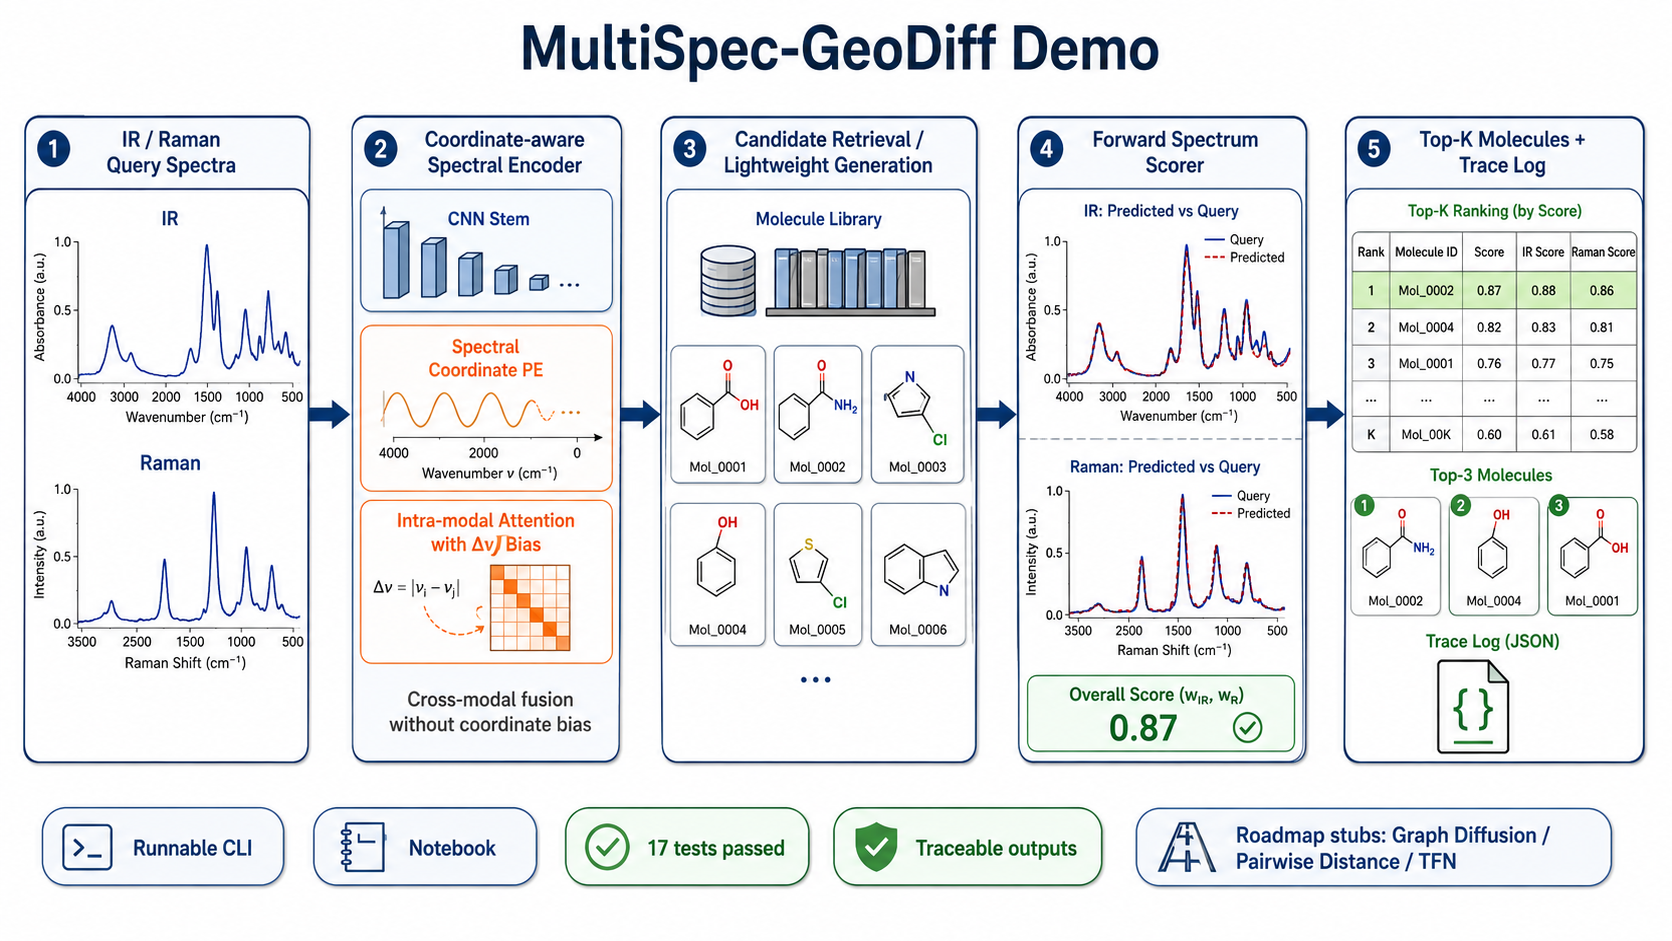
\includegraphics[width=0.84\linewidth]{figures/fig1_final_demo_pipeline.png}\\[-0.28em]
{\small 图 \thefigure：已实现 MVP 的核心闭环：IR/Raman 谱图经过坐标感知编码、候选召回与前向一致性重排后，输出 Top-K 候选、可视化结果与 trace log。}
\end{center}

\sectitle{3. 核心技术路径}
\textbf{A. 已实现 MVP}
\begin{itemize}
  \item multi-modal IR/Raman input，spectral coordinate PE，模态内 $\Delta\nu$ relative distance bias attention；
  \item cross-modal fusion（不显式加入 coordinate bias）、candidate retrieval / lightweight generation；
  \item forward spectrum scorer + reranker，输出 Top-K、attention heatmaps 与 trace log。
\end{itemize}
\textbf{B. 后续扩展模块}
\begin{itemize}
  \item size-adaptive graph diffusion；
  \item pairwise distance as 2D-to-3D bridge；
  \item parity-aware TFN-Transformer 与 chiral / tensor spectra。
\end{itemize}

\begin{center}
\refstepcounter{figure}
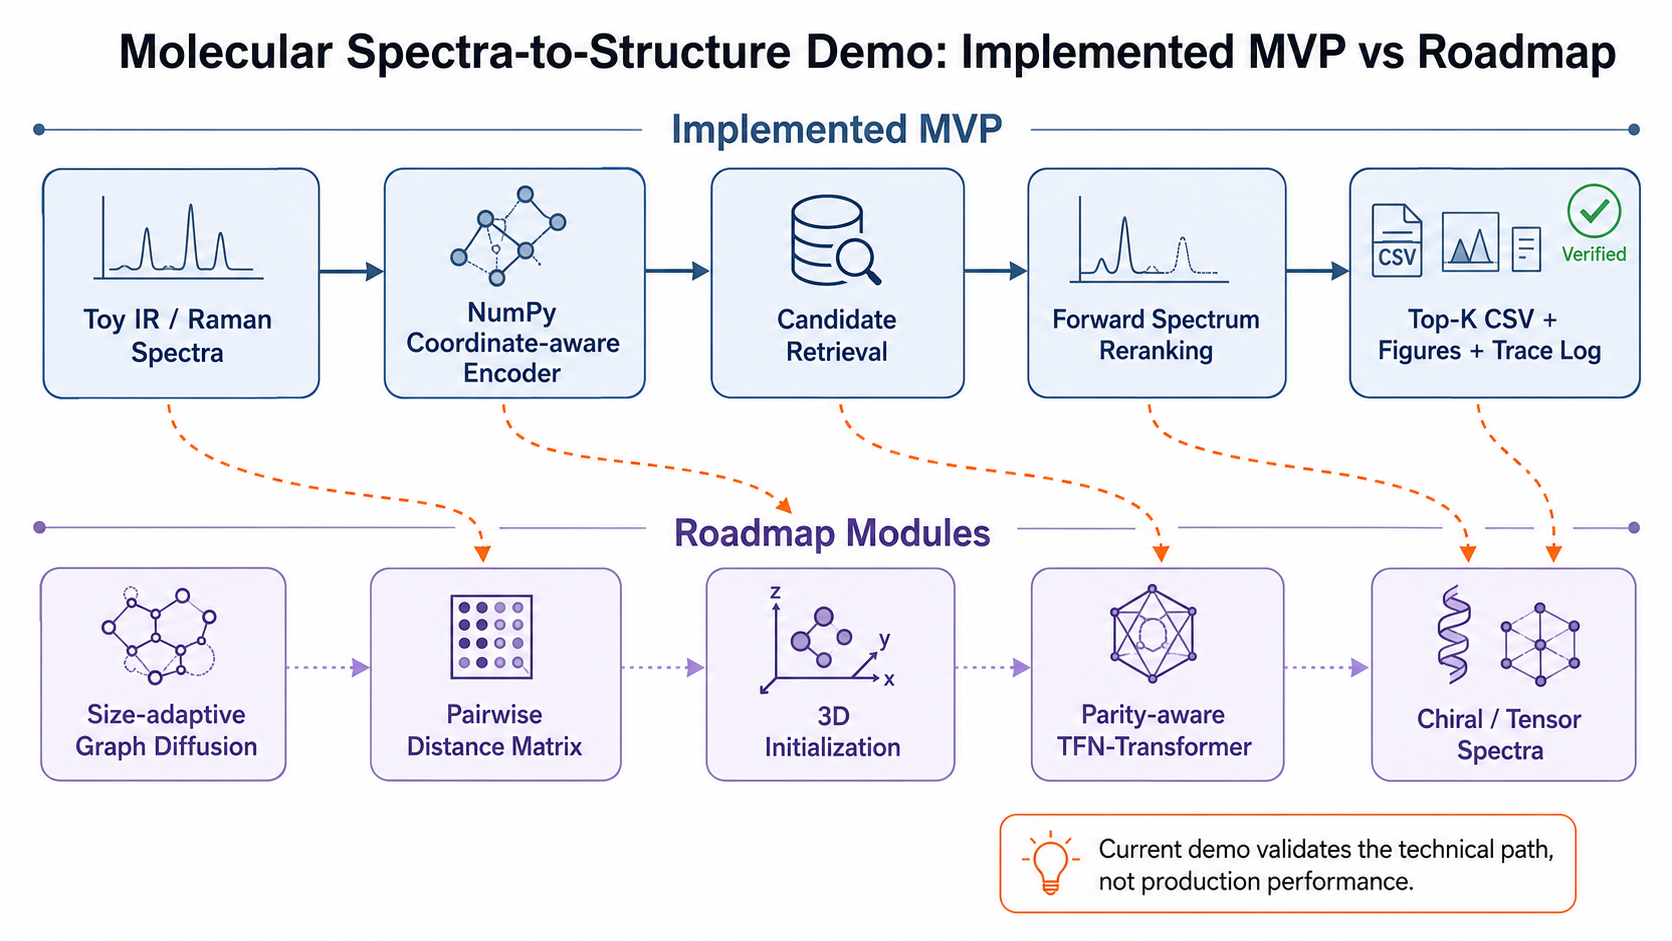
\includegraphics[width=0.78\linewidth]{figures/fig2_implemented_vs_roadmap.png}\\[-0.28em]
{\small 图 \thefigure：当前实现与后续路线的边界：当前 demo 已完成可运行 MVP；graph diffusion、pairwise distance 与 parity-aware TFN-Transformer 仍是 roadmap 接口。}
\end{center}

\sectitle{4. 可行性与验证}
\begin{table}[h]
\centering
\scriptsize
\setlength{\tabcolsep}{3pt}
\renewcommand{\arraystretch}{1.08}
\begin{tabularx}{\linewidth}{>{\bfseries}p{0.11\linewidth}X X}
\toprule
维度 & 当前实现 & 验证结果 \\
\midrule
数据 & toy IR/Raman samples + 12-molecule candidate library & sample pipeline runs end-to-end \\
编码 & NumPy coordinate-aware spectral encoder, $\Delta\nu$ attention bias & attention heatmaps generated \\
候选与重排 & candidate retrieval + forward-spectrum scoring & \cmd{topk_candidates.csv} generated \\
可追踪性 & \cmd{trace_log.json} 记录 inputs、config、scoring、outputs、fallback & validation passed \\
工程质量 & CLI、notebook、pytest、validation script & demo passed, validation passed, 17 tests passed \\
风险边界 & roadmap stubs for graph diffusion / distance / TFN & limitations documented; no overclaiming \\
\bottomrule
\end{tabularx}
\end{table}

\sectitle{5. 仓库与复现方式}
仓库地址：\url{https://github.com/techandscixie2005/MultiSpec-GeoDiff-Demo}。复现命令为 \cmd{python scripts/run_demo.py --config configs/demo.yaml}、\cmd{python scripts/validate_outputs.py --output_dir outputs} 与 \cmd{python -m pytest -q}；notebook 位于 \cmd{notebooks/demo_pipeline.ipynb}。当前 \cmd{outputs/topk_candidates.csv}、\cmd{outputs/trace_log.json} 与配套图像文件均已生成且非空。限制方面：样例数据仍是 toy synthetic spectra，不代表真实实验 benchmark；当前环境采用 RDKit / Torch fallback；graph diffusion、pairwise distance 与 TFN-Transformer 仍为 roadmap stubs，因此本 demo 验证的是技术路径、工程闭环与可追踪性，而非 production-level performance。\par

\end{document}
